\chapter{Apresentação geral do projeto}

A quantidade de produtos eletroeletrônicos cresce cada vez mais nas residências brasileiras, conforme mostra a pesquisa realizada pelo Instituto Brasileiro de Geografia e Estatística (IBGE) em 2016. A tabela \ref{ibge} apresenta a presença em números percentuais de alguns eletrodomésticos nos lares brasileiros.

\begin{table}[H]
   \caption{Presença dos produtos eletroeletrônicos nos domicílios brasileiros}
   \label{ibge}
{
   \begin{tabular}{lllll}
   \toprule
   Produto & 2012 & 2013 & 2014 & 2015 \\
   \midrule \midrule
   
    Fogões & 98,75\% & 98,76\% & 98,81\% & 98,84\% \\
    Televisores & 97,20\% & 97,16\% & 97,14\% & 97,14\% \\
    Refrigeradores & 96,65\% & 97,21\% & 97,56\% & 97,83\% \\
    Rádio & 80,86\% & 75,71\% & 72,08\% & 69,23\% \\
    Máquinas de lavar & 55,14\% & 57,46\% & 58,68\% & 61,14\% \\
    Freezer & 16,66\% & 17,05\% & 16,48\% & 16,88\% \\
   
   \bottomrule
   \end{tabular}
}{
   \legend{Fonte: IBGE 2016}
}
\end{table}

Junto com o crescimento de produtos deste segmento, o acesso à internet também cresceu muito nos últimos anos. Em matéria do portal G1 de 06 de Abril de 2016\footnote{http://g1.globo.com/tecnologia/noticia/2016/04/internet-chega-pela-1-vez-mais-de-50-das-casas-nobrasil-mostra-ibge.html acessado em 14/11/2017}, é destaque a quantidade de casas com acesso a internet, 50 por cento em média. Estes números acabam fortalecendo um outro mercado que nasce quase como uma consequência do consumo de eletrônicos e acesso a internet, o mercado de automação residencial.
Automação residencial, ou domótica, segundo o Departamento de Informática (DIN) da Universidade Estadual de Maringá (UEM) pode ser definido como:
\begin{citacao}
O termo domótica, é uma fusão da palavra latina domus (casa) e do moderno robótica. A domótica, que também pode ser referenciada por expressões como "smart building", "intelligent building", "edifícios inteligentes", é um novo domínio de aplicação tecnológica, tendo como objetivo básico melhorar a qualidade de vida, reduzindo o trabalho doméstico, aumentando o bem estar e a segurança de seus habitantes e visa também uma utilização racional e planejada dos diversos meios de consumo. A domótica procura uma melhor integração através da automatização nas áreas de segurança, de comunicação e de controle, e gestão de fluídos. \cite{DOMOTICA}
\end{citacao}

Com base nas definições conceituais anteriores, é correto afirmar que a domótica cuida da integração de sistemas e tem por finalidade tornar o ambiente doméstico e os diversos equipamentos que fazem parte dele mais fáceis de serem utilizados por qualquer morador da casa, com ou sem conhecimentos especializados em tecnologia da informação. Investir em automação residencial garante praticidade e objetividade no dia a dia sem prejudicar o conforto e segurança\footnote{http://overbr.com.br/artigos/por-que-investir-em-automacao-residencial acessado em 14/11/2017}. Este mercado oferta diversas possibilidades, como o desenvolvimento de sistemas personalizados para atender necessidades específicas, a busca por redução de consumo energético ou ainda a preocupação com a segurança podem ser a motivação para busca de soluções nesta área. Analisando um mercado maior que o nosso e que normalmente dita as tendências de futuro, a Associação Brasileira de Automação Residencial e Predial (AURESIDE) destaca:

\begin{citacao}
Pesquisas da Parks Associates mostram que mais de 100 milhões de lares dos EUA não tinham um dispositivo doméstico inteligente no final de 2016. Analistas da empresa internacional observam que alcançar essas famílias exige investimentos contínuos para criar experiências únicas e personalizadas para os moradores... 
A empresa de pesquisa, em seu serviço NUMBERS, estima que até 2020,mais de 12 milhões de lares americanos terão um detector inteligente de vazamento de água, mais de 40 milhões terão um termostato inteligente, quase 50 milhões terão uma lâmpada inteligente e cerca de 14 milhões terão um controlador doméstico inteligente. A Conferência CONNECTIONS deste ano examinará as oportunidades de investimento no IOT que impulsionarão esse crescimento e sua adoção em soluções domésticas inteligentes. \cite{MERCADO}.
\end{citacao}

Diante deste cenário promissor, soluções mais acessíveis precisam ser criadas pensando na realidade brasileira. Falar sobre ter uma opção acessível não está ligado somente as questões financeiras, embora estas tenham um peso significativo na escolha. Facilidade de obter os componentes, configurá-los e integrar isso com padrões existentes são o diferencial deste projeto.

Este projeto apresenta uma solução para automação residencial, baseada em padrões abertos que não dependem do pagamento de licensas ou direitos autorais, o que facilita a integração com outros sistemas ou dispositivos. Também utiliza componentes eletrônicos de fácil acesso e com preços razoáveis, levando em conta as soluções existentes de mercado nacional.

\begin{figure}[H]
\caption{\label{domotica} Possibilidades da domótica nos dias de hoje}
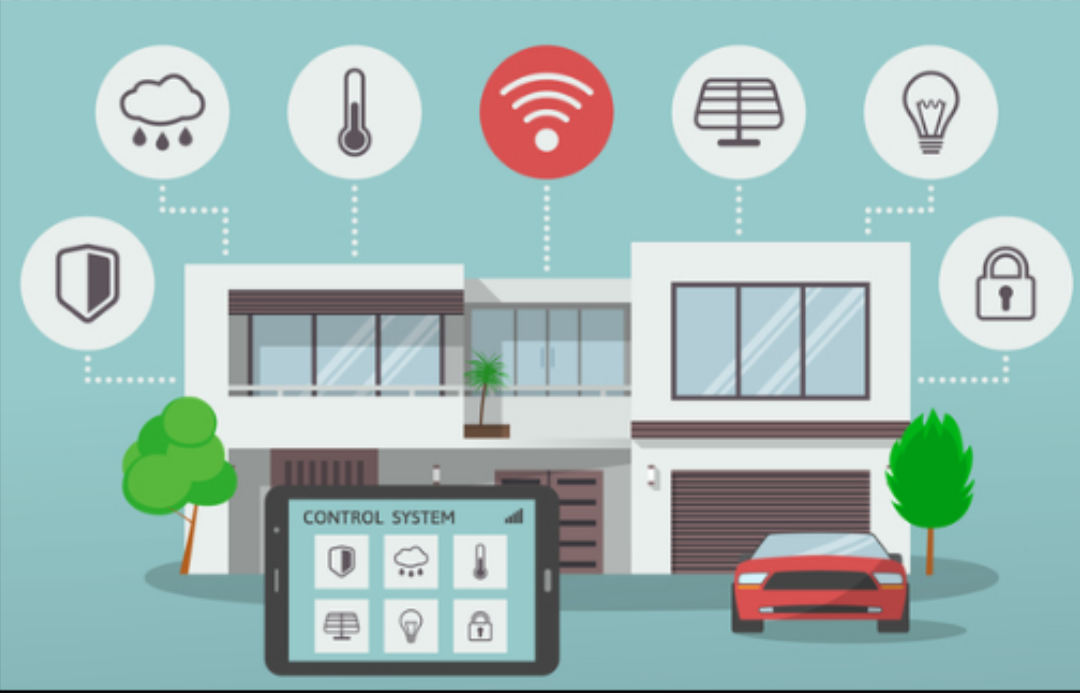
\includegraphics[scale=0.20]{img/casa-conectada.png}
\legend{Fonte: Website da Aureside \cite{MERCADO}}
\end{figure}

 A Figura \ref{domotica} mostra, de forma esquemática, as possibilidades disponíveis com um sistema de domótica em nossas residências. Possibilidades estas que vão do controle de acesso a residencia, monitoramento de áreas específicas, controle do ambiente através de sensores de temperatura ou ainda a integração com outros dispositivos inteligentes como um aparelho de TV ou central de multimídia.
